\chapter{Análisis de requerimientos}
\label{cap:analisis}

En este capítulo se identifica el proceso de selección de software para el proyecto así como el análisis de los requerimientos técnicos y funcionales.

\section{Proceso de selección de software}

Parte importante para llegar a la solución propuesta fue la selección del
software en el cual se desarrolló el nuevo proceso ETL \footnote{Extracción,
  Transformación y Carga (\emph{load} en Inglés).}. La selección de software
requirió de varios pasos previos a la toma de la decisión. El proceso de
selección de software de acuerdo a la metodología de Accenture fue la siguiente:

\begin{enumerate}
\item Establecer los requerimientos de negocio.
\item Establecer los requerimientos de evaluación de las herramientas de ETL.
\item Generar una lista larga de proveedores.
\item Generar una lista corta (generalmente 3 o 4 prveedores) de candidatos.
\item Realizar  un RFP (Request For  Approval) para evaluar a  los candidatos de
  manera individual y detallada.
\item Realizar la recomendación final del producto.
\end{enumerate}

Este proceso se datalla en la figura~\ref{fig:proceso}:

\begin{figure}[htb]
  \begin{center}
    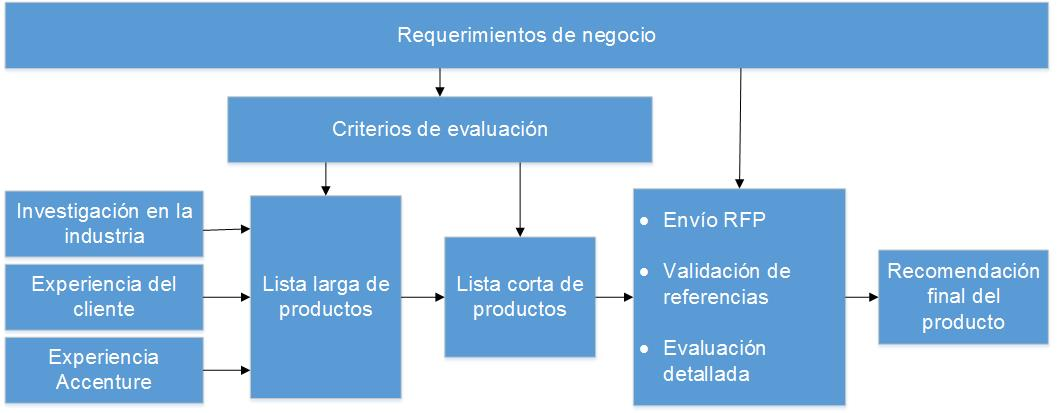
\includegraphics[width=12cm, height=3cm, scale=0.5]{Proceso_seleccion_software.jpg}
    \caption{Proceso de selección de software}
    \label{fig:proceso}
  \end{center}
\end{figure}

En las siguientes secciones se definirán cada uno de los pasos del proceso
seguidos.

\subsection{Requerimientos funcionales}

Con base en las reuniones realizadas con el área de desarrollo de sistemas de la
institución financiera se identificaron una serie de requerimientos funcionales
detallados a continuación.

\begin{itemize}

\item Se requería una conexión a correo electrónico mediante le protocolo SMTP
  para envío de informes de termino de procesos o de error en los mismos.

\item Tener un log de procesos que tuviera la información de cada uno de los
  procesos de extraccón/carga (inicio, fin, estatus de termino, errores (en cso
  de haberlos)).

\item La herramienta debía de tener la capacidad de contar con un esquema de
  limpieza de datos que permitiera identificar y corregir los errores en
  nombres, direcciones, RFC's, números de teléfono, y algunos otros datos
  relevantes para la institución financiera.

\item Permitir invocar a la herramienta ETL desde otras aplicaciones tales como
  PeopleSoft, aplicaciones desarrolladas en Java y .NET.

\item Permitir control y detalle de los errores presentados en los procesos o en
  cada uno de los componentes del flujo de datos. El control se llevaría a cabo
  mediante el envío, por parte del ETL, de errores a tablas log o archivos de
  texto en dode se pudieran identificar de una manera sencilla, los errores
  presentados.

\item Contar con un esquema de datos redundante, como puede ser un cluster,
  bases de datos replicadas, balanceo de cargas con tolerancia a fallos, etc.

\item Contar con un esquema de control de versiones que soporte el trabajo de
  multiples usuarios al mismo tiempo.

\item La herramienta debía tener la capacidad para entregar diferentes archivos
  a los sistemas destino (archivos de texto, tablas en base de datos, XML, PDF,
  Excel).

\item Contar con un esquema de seguridad basado en roles y jerarquías de usuario
  que permitieran a los usuarios acceder a datos específicos de la base de datos
  de acuerdo a su rol.

\item Contar con pantallas de configuración que permitieran a los
  administradores de la herramienta tener un mayor control sobre los procesos y
  los usuarios. Así mismo, que fuera una herramienta visualmente fácil de usar.

\item Permitir a la nueva herramienta la convivencia con las tecnologías con las
  que contaba la institución financiera (Windows 2003, SQL Server 2005, Oracle,
  DB2, AS400, Windows Vista y Mainframes)

\item Contar con una herramienta de fácil manejo de metadatos.

\item Contar con un ambiente de diseño y desarrollo 100\% visual que permitiera
  a los desarrolladores implementar las soluciones de extracción y carga de una
  manera sencilla.

\item Permitir la operación y administración de la herramienta de una forma
  remota.

\item Generar componentes reutilizables entre aplicaciones y entre procesos.

\item La herramienta debía permitir a los usuarios, la creación de funciones
  personalizadas que cumplieran con los estándares de la empresa y que no fueran
  parte de las configuraciones predefinidas de la herramienta.

\item Capacidad para calendarizar procesos; es decir, la herramienta debería ser
  capaz de ejecutar los procesos de forma automática a la hora y día
  especificados.

\item Soportar modelos de minería de datos que ayudarían a la institución
  financiera a realizar un anaálisis de sus datos y poder definir estrategias de
  mercado para los diferentes productos que ofecían.

\item Capacidades de soporte para DataWarehouse y Business Intelligence, este
  requerimiento era para cumplir con el plan estratégico de la institución.

\item Capacidad de la herramienta para plublicar procesos como Web Services a
  fin de poder acceder a ellos de manera remota o ejecutarlos a través de un
  portal con los permisos correspondientes.

\item Capacidades de detección y correción de errores en los procesos, mediante
  un proceso de depuración (Debugging) que sería ejecutado paso a paso.

\item Como un requerimiento básico, la herramienta debería de almacenar la
  información extraída en una sola fuente de datos, para la solución propuesta
  fue una base de datos de paso llamada base de datos stage.

\item Explotación de la información de una base centralizada para realizar
  reportes.

\item Consulta de datos históricos, en especial de transacciones, para poder ser
  explotados desde otro ambiente o aplicación existente en la institución
  financiera.

\item La herramienta debería de ser capaz de obtener solamente la información
  que tuvo cambios entre los diferentes periodos de extracción, ayudando al
  rendimiento del proceso y extrayendo una cantidad menor de datos.
\end{itemize}

\subsection{Requerimientos técnicos}

Por su parte los requerimientos técnicos solicitados por la institución para
seleccionar la herramienta fueron los siguientes:

\begin{itemize}

\item Mejorar el rendimiento de la extracción de datos de 90 minutos a 45
  minutos (tiempo tentativo) con una cantidad de 6 millones de registros

\item Mejorar el tiempo de transformación de datos utilizando componentes para
  limpieza y calidad de los datos.

\item Mejorar el rendimiento de la herramienta cuando el volumen de datos exceda
  los 100 millones de registros.

\item Que la arquitectura de la herramienta fuera compatible con la arquitectura
  de la institución y la futura que se planteó en el presente proyecto.

\item La herramienta debía ser capaz de poder integrarse son los sistemas de la
  institución (PeopleSoft, Core bancario, systema de reportes, sistema de
  recursos humanos, pagos a terceros, etc.)

\item La herramienta debía ser capaz de ejecutarse en diferentes paltaformas
  (Windows, Linux, Unix, Mainframes).

\item Conectividad con los istemas fuentes (ODBC, OLAP, LDAP) y con diferentes
  sistemas manejadores de bases de datos como Oracle, DB2, SQL Server, Informix,
  Sybase, Teradata.

\item Capacidad para crear funciones y métodos desde cualquier lenguaje de
  programación estructurado y que pudiera ser ejecutado desde la herramienta
  ETL.
\end{itemize}

Aunque el gobierno de datos no era parte del alcance del proyecto, pero si de la
estrategia de crecimiento de la institución, la herramienta debería de soportar
esta funcionalidad.

\subsection{Requerimientos de limpieza de datos}

Como parte de la definición de requerimientos funcionales que debía cumplir la
herramienta, existe una sección que tenía que ver con la calidad y limpieza de
datos; estos requerimientos solicitados por parte del área de tecnoloía fueron
los siguientes:

Se requería que el proceso ETL realizara la limpieza de datos de los campos
descritos a continuación:

\begin{itemize}

\item RFC. Se requería que el RFC se encontrara estandarizado y cumplieran con
  los requerimientos establecidos por el buró de crédito

\item Nombres de socios. Se requería que los nombres de socios no tuvieran
  caracteres especiales como puntos, comas, retornos de carro, paréntesis,
  corchetes, porcentaje, comillas y caracteres de 16 bits.

\item Fechas de morosidad. Se solicitó que las fechas para el cálculo de la
  morosidad se encontraran en un formato de fecha correcto yyyymmdd y que no se
  permitieran valores nulos o negativos para este tipo de dato.

\item Direcciones de socios. Fue requerido que las direcciones de los socios
  tuvieran una nomenclatura estándar para nombres de calles, colonias

\item Ciudades/Municipios. Los códigos y nombres de ciudades y municipios debían
  de contar con un estándar y estos deberian de estar corregidos de a cuerdo a
  la información proporcionada por SEPOMEX.

\item Teléfonos. Los teléfonos de los clientes debían contar con la clave lada y
  todos tenían que ser de 10 dígitos para números fijos y de 13 dígitos para
  números celulares

\item Los números telefónicos no deberían de tener guiones o caracteres
  especiales.
\end{itemize}

Como parte de la estandarización de direcciones era requerido que todos los
códigos postales se encontraran conforme a la lista proporcionada por SEPOMEX y
todos deberían de ser de 5 dígitos.

\section{Criterios de evaluación}

Como mencionamos al inicio del documento, parte importante de la selección de sofware fue la definición de los criterios de evaluación de la herramienta ETL a utilizar como parte del proyecto. Dichos criterios nos ayudaron a realizar una evaluación objetiva de las diferentes herramientas y tener un panorama general de los productos que cumplían con las caracteristicas y necesidades de la institución financiera. Tomando como base esas necesidades y la experiencia de Accenture se definieron los criterios de selección de software.

Los criterios se agruparon en conceptos genericos que describen la funcionalidad
de cada área. Estos criterios se listan a continuación:

\begin{enumerate}
\item \textit{Capacidades del servicio.}
\item \textit{Opciones de integración.}
\item \textit{Ambiente de la herramienta.}
\item \textit{Soporte y capacitación.}
\item \textit{Técnicas adicionales de integración de datos.}
\item \textit{Manejo de la información.}
\item \textit{Estrategias del producto.}
\item \textit{Estrategias corporativas.}
\item \textit{Costos.}
\item \textit{Convenios con otros proveedores.}
\item \textit{Finanzas de la compañia.}
\end{enumerate}

\subsection{Lista de proveedores}

Una vez que se definieron los criterios de evaluación y se realizó el análisis
de requerimientos con el equipo de la institución financiera, el siguiente paso
fue dar una lista larga de proveedores candidatos para ser evaluados y que en
ese momento eran las mejores opciones dentro del mercado. La lista contenía a 6
proveedores de software: Oracle (Oracle Warehouse Builder), Informática (Power
Center), IBM (Infosphere Information Server), Microsoft (Integration Services
(SSIS), SAP (SAP-Business Objects), SAS Institute (SAS).

\subsection{Evaluación de proveedores}

Con la lista larga de proveedores definida, la siguiente tarea que se llevó a
cabo fue la evaluación de cada uno de los proveedores con el fin de establecer
un grupo reducido de candidatos que representaría la lista final de selección de
la herramienta ETL a utilizar dentro del proyecto. De acuerdo a las necesidades
de la Institución financiera se definieron los siguientes porcentajes para los
criterios de evaluación

\begin{table}[htbp]
  \begin{center}
    \begin{tabular}{|p{6cm}|>{\centering\arraybackslash}m{3cm}|c|}
      \hline
      Criterio & Porcentaje de evaluación & Prioridad\\
      \hline
      Capacidades del servicio & 14\% & 1 \\
      \hline
      Manejo de la información & 14\% & 2\\
      \hline
      Opciones de integración & 11\% & 3\\
      \hline
      Ambiente de la herramienta & 11\% & 4\\
      \hline
      Costos & 11\% & 5\\
      \hline
      Soporte y capacitación & 9\% & 6\\
      \hline
      Estrategias del producto & 6\% & 7\\
      \hline
      Convenios con otros proveedores & 6\% & 8\\
      \hline
      Técnicas adicionales de integración de datos & 6\% & 9\\
      \hline
      Estrategias corporativas & 6\% & 10\\
      \hline
      Finanzas de la compañia proveedora & 6\% & 11\\
      \hline
    \end{tabular}
    \caption{Porcentajes y prioridades de evaluación.}
    \label{tab:porcentajes-y-prioridades-de-evaluacion}
 \end{center}
\end{table}

La prioridad de cada uno de los criterios de evaluación se realizó con base en
las necesidades de la institución y basados también en la funcionalidad de cada
uno de ellos.

Con toda la información que se recolectó, realicé un análisis de cada proveedor
y su herramientas presentadas, así como sus factores diferenciales y las
características principales soportadas. Esta evaluación se presenta en la
siguiente tabla con los resultados finales:

\begin{table}[htbp]
  \begin{center}
    \scalebox{0.75}[0.65]{
      \begin{tabular}{|p{5.5cm}|>{\centering\arraybackslash}m{1.7cm}|c|c|c|c|c|c|}
        \hline
        & & \rotatebox{90}{Microsoft SSIS}
        & \rotatebox{90}{Oracle OWB}
        & \rotatebox{90}{Informática Power center}
        & \rotatebox{90}{IBM IIS}
        & \rotatebox{90}{SAP\-Business Objects}
        & \rotatebox{90}{SAS} \\
        \hline
        & Porcentaje&&&&&&\\
        \hline
        \rowcolor[gray]{0.9}\textbf{Capacidades del servicio}
        & \textbf{14.29\%}
        & \textbf{3}
        & \textbf{3.5}
        & \textbf{4.5}
        & \textbf{4}
        & \textbf{3.75}
        & \textbf{4} \\
        \hline
        \rightline{Escalabilidad y rendimiento} & & 4 & 4 & 5 & 5 & 4 & 4 \\
        \hline
        \hspace{0.5cm}Alta disponibilidad & & 4 & 3 & 4 & 4 & 4 & 3 \\
        \hline
        \rightline{Seguridad} & & 3 & 4 & 5 & 3 & 4 & 5 \\
        \hline
        \hspace{0.5cm}Plataformas de ejecución soportadas
        & & 1 & 3 & 4 & 4 & 3 & 4 \\
        \hline
        \rowcolor[gray]{0.9}\textbf{Opciones de integración}
        & \textbf{11.43\%}
        & \textbf{3}
        & \textbf{3}
        & \textbf{4}
        & \textbf{4}
        & \textbf{3.4}
        & \textbf{3.6}\\
        \hline
        Conectividad con sistemas fuente & & 4 & 3 & 5 & 5 & 5 & 5\\
        \hline
        Conectividad para la carga & & 4 & 3 & 5 & 5 & 5 & 5\\
        \hline
        Servicios Web & & 4 & 4 & 5 & 5 & 3 & 3\\
        \hline
        Conexión a correo electrónico & & 1 & 1 & 1 & 1 & 0 & 1\\
        \hline
        Reusabilidad & & 2 & 4 & 4 & 4 & 4 & 4 \\
        \hline
        \rowcolor[gray]{0.9}\textbf{Ambientes de la herramienta}
        & \textbf{11.43\%}
        & \textbf{3.2}
        & \textbf{4}
        & \textbf{4.4}
        & \textbf{4.2}
        & \textbf{4.4}
        & \textbf{3.6} \\
        \hline
        Visualización del ambiente de diseño y desarrollo
        & & 4 & 4 & 4 & 4 & 4 & 4 \\
        \hline
        Manejo de errores & & 4 & 4 & 5 & 4 & 5 & 4\\
        \hline
        Ambiente de colaboración & & 2 & 4 & 4 & 4 & 4 & 3\\
        \hline
        Manejo y modelado de datos y metadatos & & 2 & 4 & 4 & 4 & 4 & 4 \\
        \hline
        Administración & & 4 & 4 & 5 & 5 & 5 & 3\\
        \hline
        \rowcolor[gray]{0.9}\textbf{Soporte y capacitación}
        & \textbf{8.57\%}
        & \textbf{4.25}
        & \textbf{4.75}
        & \textbf{4.25}
        & \textbf{4.5}
        & \textbf{3.75}
        & \textbf{4.75}\\
        \hline
        Soporte & & 4 & 5 & 5 & 5 & 5 & 4 \\
        \hline
        Capacitación & & 4 & 5 & 3 & 5 & 3 & 5 \\
        \hline
        Documentación & & 4 & 4 & 5 & 5 & 3 & 5 \\
        \hline
        Soporte a diferentes lenguajes & & 5 & 5 & 4 & 3 & 4 & 5 \\
        \hline
        \rowcolor[gray]{0.9}\textbf{Técnicas adicionales de integración de
        datos}
        & \textbf{5.71\%}
        &\textbf{ 4}
        & \textbf{2.5}
        & \textbf{4}
        & \textbf{3.5}
        & \textbf{3.5} & \textbf{1} \\
        \hline
        EII & & 3 & 3 & 4 & 4 & 3 & 0 \\
        \hline
        Cambio en la captura de datos & & 5 & 2 & 4 & 3 & 4 & 2 \\
        \hline
        \rowcolor[gray]{0.9}\textbf{Manejo de la información}
        & \textbf{14.29\%}
        & \textbf{3.6}
        & \textbf{3.8}
        & \textbf{4.4}
        & \textbf{4}
        & \textbf{3.4}
        & \textbf{3.2} \\
        \hline
        Reglas de transformación & & 3 & 3 & 4 & 4 & 3 & 3 \\
        \hline
        Perfiles de datos & & 5 & 5 & 4 & 5 & 4 & 4 \\
        \hline
        Calidad de datos & & 4 & 3 & 4 & 5 & 4 & 4 \\
        \hline
        Visualización de datos & & 2 & 4 & 5 & 2 & 4 & 4 \\
        \hline
        Contenido no estructurado & & 4 & 4 & 5 & 4 & 2 & 1 \\
        \hline
        \rowcolor[gray]{0.9}\textbf{Estrategias de producto}
        & \textbf{5.71\%}
        & \textbf{4}
        & \textbf{4}
        & \textbf{4}
        & \textbf{5}
        & \textbf{5}
        & \textbf{3}\\
        \hline
        \rowcolor[gray]{0.9}\textbf{strategias corporativas}
        & \textbf{5.71\%}
        & \textbf{3}
        &\textbf{ 3}
        & \textbf{4}
        & \textbf{3.5}
        & \textbf{3}
        & \textbf{3}\\
        \hline
        Contibución del producto & & 3 & 3 & 5 & 3 & 3 & 3 \\
        \hline
        Porcentaje de ganancias & & 3 & 3 & 3 & 4 & 3 & 3 \\
        \hline
        \rowcolor[gray]{0.9}\textbf{Costos}
        & \textbf{11.43\%}
        & \textbf{4.2}
        & \textbf{3.8}
        & \textbf{2.4}
        & \textbf{2.4}
        & \textbf{3.2}
        & \textbf{2.4}\\
        \hline
        Promedio del percio de venta & & 5 & 5 & 1 & 1 & 2 & 2 \\
        \hline
        Estructura de precios & & 3 & 3 & 1 & 1 & 3 & 1 \\
        \hline
        Modularidad de precios & & 5 & 5 & 5 & 5 & 5 & 5 \\
        \hline
        Pruebas de concepto & & 3 & 3 & 3 & 3 & 3 & 3 \\
        \hline
        Esquema de licenciamiento & & 5 & 3 & 2 & 2 & 3 & 1 \\
        \hline
        \rowcolor[gray]{0.9}\textbf{Convenios con otros proveedores}
        & \textbf{5.71\%}
        & \textbf{2.66}
        & \textbf{3.33}
        & \textbf{3.33}
        & \textbf{4.33}
        & \textbf{2.66}
        & \textbf{1.66}\\
        \hline
        Licenciamiento de terceros & & 1 & 2 & 4 & 5 & 2 & 1 \\
        \hline
        Venta del producto por terceros & & 5 & 3 & 3 & 3 & 3 & 2 \\
        \hline
        Integradores de sistemas & & 2 & 5 & 3 & 5 & 3 & 2 \\
        \hline
        \rowcolor[gray]{0.9}\textbf{Finanzas de la compañia}
        & \textbf{5.71\%}
        & \textbf{4}
        & \textbf{3}
        & \textbf{4.66}
        & \textbf{4.33}
        & \textbf{4.33}
        & \textbf{5}\\
        \hline
        Ganancias & & 3 & 2 & 5 & 5 & 3 & 5 \\
        \hline
        Crecimiento de ganancias & & 4 & 2 & 4 & 3 & 5 & 5 \\
        \hline
        Estatus del procveedor & & 5 & 5 & 5 & 5 & 5 & 5 \\
        \hline
        Total
        & 100.00\% & 168.91 & 171.18 & 190.45 & 186.76 & 172.65 & 158.21 \\
        \hline
        \rowcolor[gray]{0.9}\textbf{Calificación total}
        & & \textbf{3.54}
        & \textbf{3.52}
        & \textbf{4.0}
        & \textbf{3.98}
        & \textbf{3.67}
        & \textbf{3.20} \\
        \hline
      \end{tabular}}
    \caption{Evaluación de proveedores.}
    \label{tab:evaluacion-de-proveedores}
  \end{center}
\end{table}

\section{Lista corta de proveedores}

Con base en los criterios de selección y al análisis de las capacidades de cada
una de las herramientas, se obtuvo la lista corta de los proveedores. Los
proveedores seleccionados fueron los siguientes:

\begin{itemize}
\item IBM
\item Informática
\item Oracle
\item Microsoft
\end{itemize}

Si bien SAP-Business objects tenía una calificación mayor, el negocio decidió no
incluirlo en la lista final debido a que no se contaba con capacitación
suficiente de parte del proveedor. Así mismo, Microsoft se incluyó a petición
explicita de la institución.

La recomendación proporcionada por Accenture fue Informática debido a que al ser
una empres independiente enfocada a la integración de datos, no estaba casado
con ninguna base de datos específica, como si lo están el resto de los
participantes , y esto permitiría una mejor integración a las necesidades de la
institución. Basados en esta recomendación la institución financiera se decidió
por esta solución para implementar sus nuevos procesos ETL.

\section{Análisis de fortalezas y debilidades}
Durante el proyecto se identificaron fortalezas así como mejoras y oportunidades de crecimiento dentro de la organización. Las fortalezas identificadas en la compañía son:

\begin{itemize}
\item Uso de una sola herramienta de ETL (Microsoft SQL 2005)
\item Plataforma empresarial estandarizada (Microsoft)
\item Las personas involucradas en el proyecto contaban con el conocimiento del negocio, aplicaciones y datos, necesarios para el desarrollo del mismo.
\item Se tiene una claridad en las necesidades del negpocio e inclusive existen iniciativas de integración, limpieza e implementación de un proceso de calidad de datos.
\end{itemize}

Por otra parte se identificaron debilidades dentro de la organización que no permiten un mejor manejo de la información y explotarla de manera correcta. Dichas debilidades se mencionan a continuación:

\begin{itemize}
\item Se requería un mayor entendimiento del proceso de extracción de información
\item Mejorar la calidad de datos que se enviaban a los sistemas destino.
\item No se contaba con un proceso de limpieza de datos en el sistema origen
\item No se tenía un proceso de identificación de errores y su correspondiente solución.
\item No se tenía un esquema de gobierno de datos ni manejo de datos maestros.
\end{itemize}

Una vez identificadas las fortalezas y debilidades dentro de la compañia a nivel funcional, también se realizó un análisis de las capacidades técnologicas con las que se contaba. Principalmente se enfocó el proyecto a las capacidades del flujo de datos, es decir, aquellas herramientas técnologicas que no permitían un flujo de datos eficiente entre en sistema central y los sistemas destino. La identificación de ventajas y desventajas dentro del flujo de datos nos permitió enfocarnos en aquellos componentes que tenían que ser atendidos de inmediato.

Las desventajas identificadas en el flujo son:
\begin{enumerate}
\item Se contaba con múltiples procesos de extracción para obtener la misma información, ocasionando que el flujo de información entre sistemas fuera más lento.
\item Se tenía una sobrecarga de los procesos en el sistema origen de datos.
\item Se teanía redundancia de información; es decir, se repetía la información extraída.
\item No se tenía un proceso estándar de calidad de los datos.
\item No se tenía documentado el mapeo de datos entre el sistema origen y el sistema destino
\item No se tenía definido el flujo de datos maestros comunes a todos los sistemas.
\end{enumerate}

Del análisis realizado se identificó que el estado final del proyecto debería de ser:

\begin{enumerate}
\item Extracción de datos del sistema central una sola vez y con un único proceso ETL.
\item Creación de un mapeo entre sistema origen y destino.
\item En fases posteriores tener un esquema de manejo de datos maestros; así como limpieza y calidad en los datos extraídos y almacenados.
\item Contar con un sistema de gobierno de datos.
\item Establecer las bases para la creación de un modelo de inteligencia de negocios alineados al plan estrátegico de la compañia.
\item Creación de un repositorio central de datos que alamcene toda la información extraída y que nos permita tener una arquitectura más robusta y centralizada para el manejo de información.
\end{enumerate}

\section{Definición de los requerimientos}

Existían varios requerimientos solicitados por los diversos colaboradores de la compañia con los cuales Accenture había conversado. Con base en las conversaciones se definieron los siguientes requerimientos tanto funcionales como técnicos.

\textbf{Requerimientos funcionales}

\begin{enumerate}
\item Analizar cada uno de los datos que están siendo extraídos de los sistemas origen por cada uno de los procesos ETL implementados en el compañia.
\item Implementar procesos de limpieza de datos durante la extracción del sistema
\begin {itemize}
\item Eliminación de carácteres especiales en los nombres de los usuarios.
\item Substitución de las abreviaturas existentes en los nombres; por ejemplo: Ma; el cuál es interpretado como María.
\item Realizar la depuración de los RFC's de los usuarios ya sea agregando o eliminando caracteres para que este sea correcto.
\end{itemize}
\item Realizar los siguientes procesos de transformación durante la extracción de datos del sistema origen
\begin {itemize}
\item Transformación del formato de fecha Juliano a formato DD/MM/AAAA.
\item Transformación del tipo de dato ( númerico, decimal, fecha, char, bi
\end{itemize}
\item dentificar cada uno de las datos que son extraídos del sistema origen por medio de otras fuentes de información con la finalidad de identificar si existe una duplicidad en los procesos de extracción.
\item Creación de un repositorio central donde sea alamacenada toda la información entraída que es requerida por los diferentes sistemas de la compañia para que desde su repositorio central se distribuya la información requerida por cada sistema.
\item Desarrollo de criterios de unificación de la información que es estraída, esto con la finalidad de optimizar los tiempos de extracción de datos que realiza cada desarrollo ETL
\item Se requiere que los 20 archivos planos requeridos sean originados por la herramienta ETL que se implementará
\item Para la generación del archivo \textit{Currency\_Exchange.txt} se requiere realizar la investigación del tipo de cambio de froma automática o con una interfaz gráfica en lugar de realizar la consulta y actualización de ese valor de forma manual de ese valor después de acceder al sitio del SAT.
\item Por necesidades del negocui y debido a que dentro del plan estrátegico de la compañia est+a previto el inicio de operaciones en otros paises, será requerido el desarrollo de catálogos de información qque tengan datos y códigos sobre el tipo de moneda, ciudades, estados, paises, y códigos postales.
\item El sistema antilavado debe realizar la carga de información contenida en los archivos planos que fueron originados con la extracción, pagos a terceros y peoplesoft  de las 08:00 horas del 
\end{enumerate}

\cleardoublepage

%%% Local Variables:
%%% TeX-master: "Tesis"
%%% End:
